% This file should contain a short summary of the aerodynamic analysis tool and models

% Summarize the physics
To model the aerostructural performance of the wing, we use OpenAeroStruct, which is an open-source tool for preliminary sizing of aircraft wings~\cite{Jasa2018a}.
OpenAeroStruct uses a vortex lattice method coupled with a 6-degree-of-freedom-per-node finite element model to analyze the aerostructural properties of aircraft wings.
These inexpensive physics-based methods enable inexpensive exploration of the wing design space.
OpenAeroStruct can be used to investigate both conventional and non-conventional wings because the physics-based analyses are not necessarily dependent on previously-gathered information from existing planes.
Additionally, OpenAeroStruct provides inexpensive derivatives for all outputs of the aerostructural analyses, which enables low-cost gradient-based optimization.

% Describe the model used by this tool that was developed for the tiltwing plane
We obtain the wingspan and root chord from Johnson et al~\cite{johnson2018concept} and use other aerostructural wing properties from similarly sized aircraft.
The relevant values used in this study are listed in Table~\ref{t:aerostruct_wing}.
We use a NACA 0015 symmetric airfoil for the wingbox cross-section.
The wingbox occupies the wing from 10\% to 70\% chord for the entire span.
We include two point masses on each half-wing to account for the loading due to the engines and propellers and the magnitude of these masses comes from the upstream propulsion sizing analyses.
We use Aluminum 2024 for the lower skin and spars and Aluminum 7075 for the upper skin and apply a safety factor of 1.5 on the yield strength of the wingbox material.
A three-view and isometric view of the aerostructural wing model are shown in Fig.~\ref{f:OAS_wing}.

% Revise this table based on the actual optimization completed
\begin{table}[!htb]
 \normalsize
 \begin{center}
  \caption{Aerostructural wing properties}
  \label{t:aerostruct_wing}
    \begin{tabular}{ l r l }
        \hline
        \textbf{Design parameter} & \textbf{Value} & \textbf{Units} \\
        \hline
        Wingspan & 52.50 & feet \\
        Root chord & 4.56 & feet \\
        Elastic modulus & 73.1 & GPa \\
        Shear modulus & 27.5 & GPa \\
        Yield strength (lower skin and spars) & 324 & MPa \\
        Yield strength (upper skin) & 503 & MPa \\
        Yield safety factor & 1.5 & -- \\
        Wingbox material density & 2810 & $\text{kg}/\text{m}^3$ \\
        \hline
    \end{tabular}
 \end{center}
\end{table}

\begin{figure}[h]
\begin{center}
 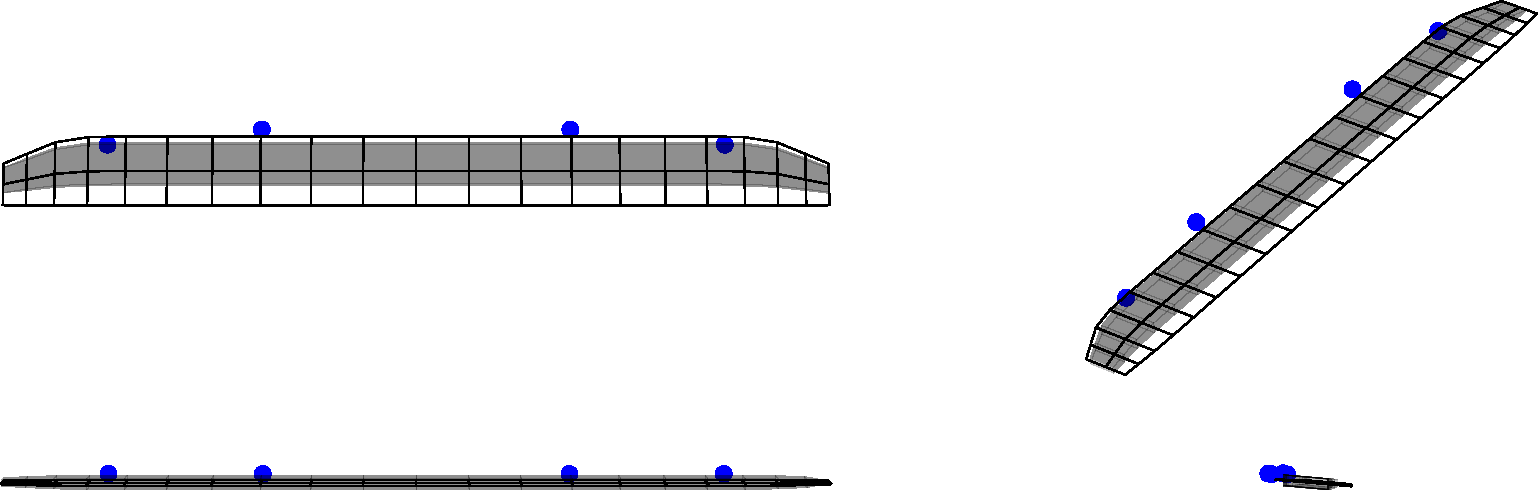
\includegraphics[width=1.0\textwidth]{../Images/aerostruct_wing}
 \caption{Three-view and isometric view of the aerostructural wing model with the engine point masses shown in blue.}
 \label{f:OAS_wing}
\end{center}
\end{figure}

We use this wing model in both the discipline design and mission performance analyses.
For discipline design, we perform a 3-point aerostructural analysis to ensure that the internal structure of the wing does not fail during limit loading.
We determine the limiting loading conditions by producing a \textit{V-n} diagram, which shows the aircraft limit load factor as a function of equivalent airspeed (EAS)~\cite{Raymer2012}.
EAS is the airspeed at sea level in a standard atmosphere where the dynamic pressure is the same as the dynamic pressure at the true airspeed~\cite{Raymer2012}.
This \textit{V-n} diagram is constructed using both the worst-case maneuver and gust loads to find the flight conditions where the wing structure is most likely to fail.
The \textit{V-n} diagram produced for this wing and nominal flight conditions is shown in Fig.~\ref{f:v_n_diagram}.
$V_S$ is the stall speed at normal level flight, $V_A$ is the corner speed, $V_B$ is the design speed for maximum gust intensity, $V_C$ is the design equivalent airspeed, $V_D$ is the design diving speed.

In this case, we use a maneuver loading of 2.5g, $V_C$ is the max cruise speed from Johnson et. al.~\cite{johnson2018concept}, and $V_D = 1.25 V_C$.
We analyze all of these limit loading flight conditions at an altitude of 5000 feet.
The gust lines are from the Federal Aviation Regulation (FAR) 25, which provide airworthiness standards for transport airplanes~\cite{far25}.
From Fig.~\ref{f:v_n_diagram}, the most critical loads are at 2.8g and --1g due to gust loading and push-over conditions respectively.
Therefore, we use 1g, --1g, and 2.8g flight conditions in the 3-point aerostructural analysis in the discipline design.

\begin{figure}
\begin{center}
 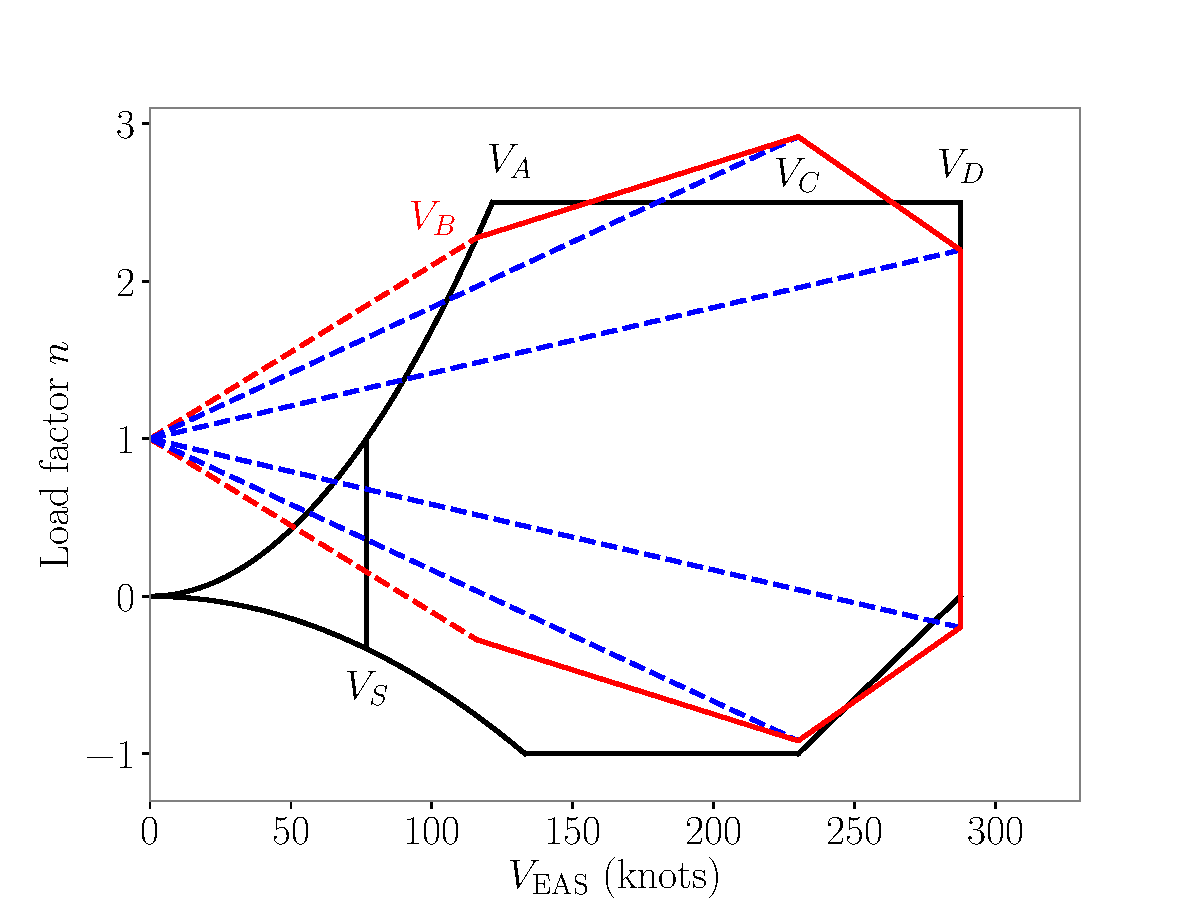
\includegraphics[width=0.6\textwidth]{../Images/v_n_diagram}
 \caption{\textit{V-n} diagram used to determine the limiting flight conditions for the wing structure.}
 \label{f:v_n_diagram}
\end{center}
\end{figure}

For the mission performance analyses, we only model the aerodynamic wing without considering the wingbox structure to lower the computational cost.
The change in aircraft performance due to changes in wing deflection across the cruise segments of the mission is negligible, which allows us to use only aerodynamic analyses in the mission performance portions of the problem.
The wing deflection obtained from the 1g aerostructural analysis is applied to the wing mesh used in the aero-only cases.
Nominally, we will not experience structurally limiting loads during the mission, so we subject the wing structure to its limit loads in the discipline design analysis portion.
